\chapter{ブロックチェーン技術}
本章では、本研究で用いるブロックチェーン技術について述べる。
最初に仕組みや説明を述べ、その技術が持つ問題点や現状の政治的な問題点について述べる。
その後、ブロックチェーン技術を最大限に活用するための技術であるオフチェーン技術について述べる。
そして、ブロックチェーン技術を用いた暗号通貨の代表的なものについて説明を行う。
最後に、本章のまとめを行う。

\section{仕組み}
本節では、ブロックチェーンの仕組みについて述べる。
また詳しくは後の\ref{3.1.4}項にて後述するが、ブロックチェーンにはいくつかの種類が存在する。
ここでは特に指定のない限り、中央集権的な機関の存在しない、パブリック型ブロックチェーンについての説明を行う。

\subsection{P2P通信}
ブロックチェーンはP2P通信によって行われる。
このP2P通信とは、対等の端末間で行われる通信のことである。
通常のネットワークサービスは、クライアント・サーバ型と呼ばれる通信機能によって運営されている。
サーバ側ではサービス運営者がサービスや機能を提供するアクセス可能なコンピュータであるサーバを設置し、このサーバ上でサービスが運営される。
例えば慶應義塾大学湘南藤沢キャンパスにて使われている学事システムのSFC-SFSでは、履修可能単位の閲覧機能、履修単位申告機能、履修者が過剰になった時の選抜機能などを提供している。
この機能を運営しているコンピュータを一般に、サーバと呼ぶ。
これに対し、利用者はクライアント側となる。
クライアントとは、サーバに対してそれが持つ機能を使わせてもらうためのリクエストを送るコンピュータのことである、
SFC-SFSの例では、学生がサービスにアクセスするために使うスマートフォンやPCなどがこれに当たる。
つまり、サービスの提供者側であるサーバと消費者側であるクライアントで役割が分かれていることが特徴だ。
このような形で通常のネットワークサービスは運営されるが、P2Pサービスはこれと異なる。
P2Pサービスでは、通信する端末間の関係が対等である。
つまり通信する双方が同じ機能を持ち、相手へサービスを提供する一方で、相手からサービスを受けているという状況が発生しているのだ。
P2Pサービスの例として、インターネット回線を使った通話アプリが存在する。
P2Pの通話サービスの場合、Aの端末とBの端末で通話を行なっている時、この通話アプリを提供している会社は二人の会話中の通信について関与していない。
双方ともが自分の音声を相手へ提供する機能と相手の音声を受け取る機能を持つ、つまりクライアント・サーバ型の両方の機能を双方が持っているのだ。
以上がP2P通信の特徴である。
ブロックチェーン技術は中央集権を持たない環境での分散台帳技術であるが、これにはP2P通信が使われている。
したがって、全ての参加者がサービスの使用者としての役割のみならず、サービスの提供者としての役割も持っているのだ。

\subsection{デジタル署名とアドレス}
デジタル署名とは、あるメッセージが署名した人によって作られたかを検証する仕組みである。
ここでは「Aが自分の3BTC(Bitcoin)を使いたい」と主張する時に、それが本当にAの発言であるかを担保するのがこのデジタル署名の役割である。
代表的なブロックチェーンであるBitcoinやEthereumではECDSA(楕円曲線DSA, Elliptic Curve Digital Signature Algorithm)を利用しており、これについて説明を述べる。
(!!!後に参照する図を挿入のこと!)
\begin{equation}
y^2 = x^3 + ax + b
\end{equation}
以上が楕円曲線について一般的に表される式である。
この中でもBitcoinやEthereumが用いる規格であるsecp256k1曲線はa=0, b=7であるため、以上の方程式は
\begin{equation}
y^2 = x^3 + 7
\end{equation}
上記のように表される。
また楕円曲線の加算の定義として、点Aと点Bを加算することを考える。
この時、加算後の座標は点Aと点Bとを通る直線のもう一つの交点のx軸に関して対称移動させた点である。
したがって点Aと点Bが同一座標の点Gであるとき、その接線と楕円曲線との交点をx軸に関して対称移動させた点は
G + G = 2G
となる。
secp256k1はGのベースポイントを定めており、そこから秘密鍵rを掛け合わせたrGが公開鍵となる。
この時、楕円曲線上の離散対数問題によって秘密鍵から公開鍵を導出することは容易であるが、逆の公開鍵から秘密鍵を導出することは難しいことが知られている。
この秘密鍵を使い、「自分のBitcoinを使いたい」と主張することによって、利用者は自分のBitcoinを使用する事が可能となる。
この主張を行う際の署名値は以下の式によって導かれる。
\begin{equation}
S=\frac{h+kR}{q}{(mod p)}
\end{equation}
\begin{list}{}{}
\item q:一回のみ使われる乱数(\(1 \leq q \leq 2^256-2^32-977\))
\item h:取引情報のハッシュ値
\item k:送信者の秘密鍵
\item R:一時的な公開鍵のx座標
\item p:楕円曲線のx座標がこれより大きくならないための値で素数
\end{list}

そしてこれらの値のうち、SとRが署名となり、ブロックチェーン上で周知される。
この主張が本人のみ知り得る秘密鍵を使って行われたものかを確認する際は、以下の式を使って検証する。
\begin{equation}
Q=\frac{hG}{S}+\frac{RK}{S}{(mod p)}
\end{equation}

\begin{list}{}{}
\item S, Q, R:送信者から受け取った署名
\item h:取引情報のハッシュ値
\item G:secp256k1のベースポイント
\item K:送信者の公開鍵
\item p:楕円曲線のx座標がこれより大きくならないための値で素数
\end{list}

以上の式において、Qのx座標が送信者が送信したRの座標と一致する時、この署名は正しいものであると検証される。
また、この公開鍵をBitcoinではHASH160\UTF{00B7}EthereumではKeccak256ベースのハッシュ関数によってそれぞれハッシュ化し、Ethereumではそのハッシュ値の末尾20バイトを抜き出したものがアドレスとして使われる。
そして「そのアドレスに対して、3BTCを送金する」と主張できるようになり、このアドレスの管理者(つまり元の公開鍵や秘密鍵を持っている者)がその後、「ここで受け取った3BTCを使う」と主張できるようになるのだ。
(!!!後に参照する図を挿入のこと!)

\subsection{トランザクション}
ここでは、Bitcoinを例にとトランザクションについて説明を行う。
ブロックチェーン上の記録は、全てトランザクションという単位毎に格納される。
つまり、「AがBに3BTCを渡した」という記録が一つのトランザクションに格納されるということだ。
このトランザクションはインプット部分とアウトプット部分、そしてその他の部分が存在する。
インプットには、当該トランザクションのトークンの出所が存在している。
例えば、「Aが3BTCを使う」と申し出たとしよう。
この時、ネットワーク全体が「Aは3BTC以上持っている」ということが分からないと、Aが3BTC使うという行為は認められない。
ここで「3BTC以上持っている」ということは、換言すると「3BTC以上を誰かから送金された過去があり、そのBTCは未だに使用されていない」ということである。
この「未だに使用されていなく、その所有者が未だ使える状態」のトランザクションのことをBitcoinではUTXO(Unspent Transaction Output)と呼ぶ。
このUTXOを使おうとする時は、トランザクションのインプットにUTXOの存在する場所を明示することで、UTXOを使う事ができる。
つまり、インプットはトランザクションの送金における払い手に当たる情報が入る部分と言える。
次に、アウトプットについて説明する。
アウトプットはトランザクションの送金における受け取り手に当たる情報が入る部分である。
前項で述べたように、受け取り手の情報はアドレスによって表される。
したがって、「AがBに3BTCを渡した」あとで未だにBがこれを使っていない状態の時、このトランザクションのアウトプットの署名欄にはBitcoinアドレスが存在している。
その後、「BがCに3BTCを渡した」とすると、先ほどBitcoinアドレスが書かれていた署名欄にはBitcoinアドレスの素となった公開鍵とこの公開鍵に対応する署名値が代入される。
つまり、あるアウトプットがUTXOであるか否かの判断はこの署名欄にBitcoinアドレスがあるか公開鍵と署名値が存在するかの違いによって行われる。
このようにしてトランザクションは管理される。

\subsection{ブロックとマイニング}
ここではブロックとマイニングについて説明を行う。
ブロックチェーン技術は情報の記録を単一の歴史を共有することによって、参加者の合意できる台帳管理を行おうとする技術である。
この単一の歴史を刻む歴史書の1ページが1ブロックに当たる。
現在のBitcoinでは10分に1回、Ethereumでは15秒に1回、それぞれのペースで新しいブロックが生成される。
このブロックにはトランザクションが0個以上含まれており、その処理内容が単一の歴史として刻まれる。
そしてブロックチェーン技術はこの方式によって、二重支払い問題を解決している。
Aが3BTCを持っている時、同時に「AがBに3BTCを払う」と「AがCに3BTC払う」というトランザクションを発行しようとしたとする。
しかし、ブロックが生成される際にのみ送金の処理は行われるため、ネットワークの遅延等の影響によって二つのトランザクションが承認されることはあり得ない。
また、各々のブロックはヘッダに前のブロック情報をまとめたハッシュ値を持っており、どのブロックの次に繋げられたブロックであるかを明示している。
このブロックがチェーンのように何個も連なることによって、ブロックチェーンという分散管理台帳が形成されていく。
そしてこのブロックが生成される際に行われることが、マイニングと呼ばれる行為である。そしてブロックの生成を行おうとする者をマイナーと呼ぶ。
ブロック情報をまとめたハッシュ値の中には、ナンスと呼ばれるブロックのマイナーが付加する32bitの数値が存在する。
このナンスを含めたハッシュ値が、一定の数だけ頭に0を持つようにすることによって、そのブロックは正当なブロックであると承認されるようになっている。
例えば、Bitcoinのメインネットワークにおいて553582番目に生成されたブロックの情報について見てみる。
以下はBitcoinの現在の統計情報などを提供しているhttps://www.blockchain.com/ja/ から取得した情報である。
すると、ハッシュ値は「0000000000000000001b0218ca2b54e9809b5d948864c5bd1e657e5aa09f438f」となっている。
そしてこの時のナンスの値は「4142738813」となっている。
ブロックの持つトランザクションのハッシュ値などの情報に、このナンス値を足したところ、このように頭にいくつもの0がつくハッシュ値を見つけ出せたのである。
この時この様々なナンスの値を取り付け、0が頭に一定数以上つくハッシュ値を見つけ出す行為について、マイニングと呼ぶ。
そしてこのマイニングという行為によって、ブロックチェーンにおける改竄可能性を防いでいるのだ。
現在(2018-12-13 00:46:30)、マイニングは16進数において頭の18文字に0が続く場合、ブロックが生成されるようになっている。
つまり、最新より一つ前のブロックのハッシュ値をブロックに含めて\(16^18\)回の演算を行うことで最新のブロックを無効にでき、自分の思い通りのブロックを提出する事ができる。
しかし、2つ前のブロックを変更しようとするときはどうだろう。
Bitcoinの各参加者は、ブロックがもっとも長く連なったブロックチェーンを信用するように設計されている。
つまり2つ前を変更するには、新しく2つ分のブロックを生成しなくてはならないのだ。
この時に必要な計算量は\(16^(18\times2) \)となり、難易度は格段に上昇する。
これがさらに3つ前、4つ前..となっていくと、事実上変更は不可能となる。
よって3BTCを払い、その対価としてのサービスを受けたのちにその支払ったBTCを取り返すために新しいブロックを作り直す行為は、ブロックが一定数以上深くなった場合においては不可能である。
つまり理論的にブロックの改竄は可能であるが、それは実際にはそれを行うことは極めて難しいということである。
これがブロックチェーンの参加者が公開台帳を信用する理由であり、改竄耐性を持つという理由である。
そしてマイナーがこのマイニングを行う動機はマイニングを成功した時に成功報酬がもらえることである。
この成功報酬はブロック高によって決められており、最初は50BTCで始まり、2018年12月現在では12.5BTCである。
このようにしてブロックは生成され、ブロックチェーンは管理される。

\section{問題点}
ここでは、前半の2項でブロックチェーン技術に関する固有の問題点を述べる。
その後、後半の2項で現在のブロックチェーン事情に関する問題点を述べる。

\subsection{スケーラビリティ}
ここではブロックチェーンで管理することによる、トランザクション処理数に関するスケーラビリティの少なさについて述べる。
Bitcoinでは1ブロックに含める事が可能なデータ量は1MBとなっている。
このデータ量の中にトランザクションに関するデータを含めなくてはならないため、1ブロックで処理できるトランザクションの数は限られている。
そしてブロックの生成ペースは平均で10分に1回になるように調整されるため、処理できるトランザクションの数は時間当たりで一定であると言える。
つまりBitcoinを100人が使おうが、100万人が使おうが、同じだけの処理能力しか存在しないのである。
例えばWebサービスであれば、受け付けるリクエストに対する処理能力を上げる方法はたくさんある。
Webサーバの台数を増やし、ロードバランサで負荷を振り分ける。
DBを分散処理させ、データモデリングを見直してよりレスポンスの速いDBにする。
JavaScriptを後から読むようにし、思い画像は最初のトップページ範囲を表示してから順にAjaxで取得する。
など、様々な方策を打てる。
しかし、ブロックチェーンは時間をかけてマイニングを行い、複数のチェーンが同時並行で存在していくことを防いでいる。
もし3秒に1回のペースでブロックが生成される場合、同じ長さのチェーンが大量にできてしまい、どれが本当の台帳とみなして良いかわからなくなる。
また、ブロックには一定のサイズしか入らないことで最新のブロックが変更された時の巻き戻されるトランザクションの数を減らしている。
もし大量のトランザクションを1つのブロックに入れた場合、それはブロックを広報する際の遅延が生じる。
この時、最新のブロックからマイニングを行いたいマイナーは、ブロックの遅延によって不利を受ける。
これが続いた場合、マイナーが少なくなり、マイナーの一極集中を招く恐れがある。
このことによる弊害については3.2.4にて後述する。
つまり、仕組みそのものに固有のスケーラブルになり得ない要素が含まれているのだ。
勿論、マイニングには参加者が多い方がマシンパワーが大きいので、変更されにくいブロックを生成する事が可能である。
しかしながら、それは改竄耐性が上がるのみであり、トランザクションの処理能力は上がらない。
どれだけ沢山の参加者が増えたとしても、それはセキュリティ性を高めるために使われてスループットを犠牲にしている、ここにブロックチェーンの大きな問題点の一つが存在する。

\subsection{手数料とマイクロペイメント}
全世界では大量のトランザクションが生成されている。
従って、生成された全てのトランザクションが直ぐに最新のブロックに入るとは限らない。
この時、早くマイナーにブロックへ入れて貰うため、トランザクションの送信元は手数料を設定することができる。
この手数料はマイナーが得る成功報酬にプラスして、マイナーへと渡る。
よって、より多くの手数料を指定した方が早くトランザクションが処理される可能性が高まるのだ。
またブロックサイズの上限が決まっているため、トランザクションの大きさが大きい程、多くの手数料がマイナーへのインセンティブに必要となる。
1MBの内500KBを使うトランザクションを処理して0.01BTCの手数料のトランザクションと、1MBの内50KBを使うトランザクションを処理して0.01BTCの手数料のトランザクションとでは残りのブロックに入れられるトランザクションの大きさが変わってくるためである。
残りでより大きなトランザクションを捌ける方が、より多くの手数料を獲得できるためである。
しかしこの仕組みは、小さな買い物に使うためには適していない。
手数料はトランザクションベースで決まるため、少額の支払いであれば手数料が少なくて済むという性質のものではないためである。
つまり、Bitcoinで10円にあたる飴を買う際も1000万円にあたる高級車を買う際も、同じ速度で処理してもらうには同じ手数料が必要なのだ。
よってここまで記したのブロックチェーン技術では、マイクロペイメント(少額取引)には適さないという問題点がある。

\subsection{マイナーの一極集中}
ブロックはブロックチェーンにおける歴史書の1ページであり、マイナーはそのブロックを承認する役割を持っている。
即ち、マイナーは取引の歴史の承認者、ブロックチェーンの管理者と換言できる。
そしてそもそも、ブロックチェーンは完全に分散された記録システムであった。
中央集権な機関が存在しないので、その完全に透明性が保たれたプラットフォームを信用する人が参加するものとして作られた。
しかしながらこの前提を覆すようなことがBitcoinでは起こったと、Bitcoinのコア開発者でBlockstreamの共同設立者であるPieter Wuille氏は言う。(http://nonem.hatenablog.com/entry/2017/10/14/182226)
マイナーの中にはマイニングプールと呼ばれるものを作り、ブロックを生成している集団がある。
彼らは自宅のPCなどでマイニングをしたいものの、成功する確率が少ないので大勢でマイニングを行っている。
そして例えば各人の計算能力が同じ100人で12.5BTCを採掘した場合は、1人あたり0.125BTCずつ分配する。
このいくつかのマイニングプール間で、生成したブロックを送信する前にブロックヘッダのみを共有しているようなのだ。
これにより、情報を共有するマイニングプールは他のマイナーよりも早くマイニングに取りかかることができる。
これは計算能力を信用しているのではなく、共有の相手のマイニングプールを社会的に信用していることであり、これはBitcoinの基本理念に反する。
それと同時に、これらのマイニングプール間でのマイニングが有利となり、他のマイナーがマイニングに参加する際に不利となってしまう。
ここで、これからマイニング参加するにはこのマイニングプールに所属する方法が一番良い方法となる可能性がある。
その際マイナーは歴史の承認者であるため、一極集中するとその間でメインのBitcoinとは別の取り決めを作ってしまい、それがBitcoinのルールとなってしまう可能性がある。
この時、本来の目的と離れてBitcoinに中央集権的な機関が存在してしまう可能性がある。
以上の理由から、マイナーの一極集中は望ましいことではなく、現在のBitcoinを取り巻く状況の問題点の一つである。

\subsection{現在のOSSブロックチェーンの運営}
"Decentralization in crypto is a myth. It is a system more centralized than North Korea: miners are centralized, exchanges are centralized, developers are centralized dictators"
「暗号通貨が中央集権的でないと言うのは神話である。そのシステムは北朝鮮よりも中央集権的である。マイナーは中央集権的で、交換所は中央集権的で、開発者は中央集権化された独裁者である。」
以上の言葉はニューヨーク大学のNouriel Roubini教授がtwitterで発言した言葉である。
確かに、現在のブロックチェーンはパブリック型であってもその仕様の決められ方は決して民主的なものではない。
Ethereumは2019年の1月にハードフォークが行われることが決まったが、これは開発者会議によって決まったものだ。
それ以前でも、EthereumはThe DAO事件の時のハードフォークから中央集権的であると批判を集めてきた。
The DAOというEthereum上で動くトークンの資金集めに150億円分のEthereumが集められた。
しかし、Ethereum上で動かすsolidityと言う言語のフォールバック関数の仕様に関しての見落としがあり、3分の1が攻撃者によって抜き取られてしまった。
その際、Ethereumコミュニティは歴史書であるブロックチェーンの巻き戻しを行い、攻撃者が利益を得ることを阻止した。
このような対策が一プロジェクトのバグに対して行われること自体が、中央集権的であることの証左である。
ここにマイナーやETH(Ethereumの通貨単位)を持っている人間の意思は反映されていない。
マイナーの件に関しては前項で述べたものがそのままこのツイートの論拠となる。
このように、現在のOSSブロックチェーンはパブリック型と謳いつつ、とても中央集権的であるという側面を持っている。

\section{オフチェーン技術}
ここではオフチェーン技術について述べる。
今までのブロックチェーンに関する説明はこれに対応してオンチェーンと呼ばれることがある。
オンチェーンはトランザクションの制限が厳しく、全世界で使われる通過の処理が10分に1回しか行われない。
Bitcoinが始まって以来、一日のトランザクションが45万を超えたことはない。
これは、秒間5.2トランザクション以上が処理されたことがない計算になる。
VISAを始めとした決済システムは遥かに多いTPS(Transaction Per Second)を実現しており、世界中の決済を目的とするには5TPSは明らかに少ない数字である。
この制約を緩やかにするため、オフチェーン技術と総称される技術が存在している。
例えば1曲100BTCで楽曲を配信するサービスを考えてみる。
最初に、ユーザは使いたいBTCをオンチェーン上にデポジットする。
10曲分配信サービスを受けたいと予定したすると、1000BTCをデポジットする契約をトランザクションとして広報する。
その後1曲の配信サービスを受けるとき、支払い側は100BTC分を払うという署名を行ったトランザクションを受け取り側へ送る。
受け取り手はこのトランザクションを確認次第、1曲の楽曲を配信する。
そして支払い側がもう1曲楽曲が欲しい時は今度は200BTCを払う署名を行ったトランザクションを受け取り側へ送る。
というこの繰り返しを行い、もう支払い側が要らないと思った時、このオフチェーンでのやり取りを終える。
この時の実際の操作としては、受け取り側が精算する旨をトランザクションとして広報することを行う。
そしてもし6曲の配信サービスを受けた時、600BTCが受け取り側に、400BTCが支払い側に支払われる。
この時、最初と最後の2つのトランザクションのみオンチェーンには広報したが、実際にはオフチェーンによって6曲分の支払いがなされている。
オンチェーンのみでは6つのトランザクションが必要なところを2つのトランザクションのみで同じ機能を提供できたということである。
これがオフチェーン技術の概略であり、これに対する細かな実装はブロックチェーンの種類によって違う。
各々がBitcoinとEthereumのオフチェーン技術の一つである、ペイメントチャネル技術とμRaiden技術については後の3.5.3項と3.6.4項にて行う。

\section{Bitcoin}
ここではブロックチェーン技術を使って作られた最初の実装物であるBitcoinについて述べる。
3.1節で説明したことと重複することが多いが、のちのEthereumと対比するために述べる。
通貨単位はBTCである。

\subsection{トランザクションベースの一元管理}
Bitcoinは全てトランザクションベースで管理される。
3.1.2項で述べたように、自分のBTCを使いたい時はそのBTCをもらった過去のトランザクションを指定する。
そしてそのトランザクションを指定してBTCを使った過去がないことを承認ノードが確認(UTXOであることを確認)した上で、そのBTCは使用される。
ここで、仮に10BTCを貰ったトランザクションを使って3BTCを使いたいとする。
すると支払い側は生成されるトランザクションは3BTCを支払い相手へ渡し、残りの7BTCは自分のアドレスへ送るように指定することで3BTCのみを使うことが可能となる。
この工夫が一般的である理由は、トランザクションベースの一元管理であることに存在する。
もし7BTCを明示しない場合、お釣りの7BTCがそのまま送信者のアドレスに紐づけられたままできるのであればトランザクションのサイズを減らし、トランザクション送信の際の手数料を少なくできる。
お釣りのアドレスを指定することは送信相手を複数指定するためにトランザクションのサイズが大きくなることを招き、このことがトランザクション送信の際の手数料増大を招くためだ。
もしアカウントベースでBitcoinが管理されていれば、この方式を行うことに一定の負のインセンティブが存在するのだ。
また、トランザクションベース管理ではこのお釣りであるという情報を秘匿する工夫も考えられている。
もし同じBitcoinアドレスへ7BTCを送った場合はこの7BTCがお釣りであることが明確であり、本来は公開されるべきでない支払い情報の一部が全世界にバラされてしまう心配がある。
よって、これに対する一般的対策としてBIP(Bitcoin Improvement Proposal)-32で提案された、拡張鍵生成が知られている。
これはチェーンコードやインデックスの数字を用い、新しく秘密鍵\UTF{00B7}公開鍵\UTF{00B7}Bitcoinアドレスを生成する方法の一般的方法である。
これを使うことで、同じく自分が管理しているアドレスでありながらマイナーや他の参加者からはどちらがお釣りでどちらが本来の支払いに使われたのか、あるいはどちらも別々の支払いに使われたのかが分からなくなる。
このようにして、支払い情報についてなるべく公開されないような工夫が一般的に行われている。
また、Bitcoinが徹頭徹尾トランザクションベースで管理されていることがこれらの振る舞いや工夫から分かる。

\subsection{script言語とチューリング不完全}
Bitcoinの署名に関して、具体的な方法について今まで言及してこなかったが、これがscript言語と呼ばれるもので行われているという具体的プロセスをここで記す。
UTXOの使用時、script言語と呼ばれる言語によって記述されたプログラムが正を返す時、そのUTXOは使用可能となる。
Bitcoinの使用例としてもっとも代表的である、Bitcoinをあるアドレスからあるアドレスへ移動させる場合を考える。
その際のプログラムは以下のようになる。
\begin{lstlisting}[caption=script言語,label=scripting]
<sig> <pubK> DUP HASH160 <pubKHash> EQUALVERIFY CHECKSIG
\end{lstlisting}
\begin{list}{}{}
\item \verb|<|sig\verb|>|:秘密鍵でトランザクションに署名したもの
\item \verb|<|pubK\verb|>|:公開鍵情報
\item DUP:一つ前の内容をコピーする命令
\item HASH160:公開鍵からアドレスをBASE58でデコードしたものを導く関数
\item \verb|<|pubKHash\verb|>|:アドレスをBASE58でデコードしたもの
\item EQUALVERIFY:スタックに積まれている一つ前ともう一つ前が同じであることを確認する命令。異なればその時点でプログラム全体の返り値がFalseとなる。
\item CHECKSIG:二つ前の署名値が一つ前の公開鍵情報に対して正しいか否かを判断する。
\end{list}

このscript言語は逆ローランド記法であり、順に命令がスタックに積まれて実行されていく。
なお、この時トランザクションのアウトプットに記述される、トランザクションをロックするためのプログラムが以下である。
\begin{lstlisting}[caption=ロックを行うscript言語,label=scripting-lock]
DUP <HASH160> <pubKHash> EQUALVERIFY CHECKSIG
\end{lstlisting}
そしてインプットに記述されるトランザクションをアンロックするためのプログラムが以下である。
\begin{lstlisting}[caption=アンロックを行うscript言語,label=scripting-unlock]
<sig> <pubK>
\end{lstlisting}
つまり、「アンロックのためのプログラム」と「ロックのためのスクリプト」をこの順番で続けて実行することでトランザクションへの署名が正しいかの判断は行われる。
以下にその時の様子を示す。
\begin{enumerate}
\item \verb|<|sig\verb|>|がスタックに積まれる
\item \verb|<|pubK\verb|>|がスタックに積まれる
\item DUPによって\verb|<|pubK\verb|>|が複製される
\item HASH160によって3番目で複製された公開鍵情報がアドレスのデコードされた状態の値になり、スタックに積まれる
\item \verb|<|pubKHash\verb|>|がスタックに積まれる
\item EQUALVERIFYによって4番目でハッシュ化されてスタックに積まれたものと5番目でスタックに積まれたものとを比較する。同じであった場合は実行中のプログラムが続行され、異なっていた場合は実行中のプログラムは中止する。
\item CHECKSIGによって、1番目でスタックに積まれた署名値と2番目でスタックに積まれた公開鍵情報を検証し、正しいものであれば真を返し、間違っていれば偽を返す。
\end{enumerate}
以上がscript言語の実行内容である。
また、このscript言語の特徴として、チューリング不完全であることが挙げられる。
このことにより、チューリング完全である時と比べてセキュリティホールが少なく済むことが知られている。
その一方で、このスクリプト言語によりユーザが望む様々な処理が実現できるとは限らない。

\subsection{ペイメントチャネル}
Bitcoinにおけるオフチェーン技術であるペイメントチャネルは、トランザクションの持つロックタイム機能とマルチシグ機能を併用して実現される。
ロックタイムとは、定めた時間になった時までそのトランザクションが実行されない機能のことである。
マルチシグとは、あるUTXOを使う際に複数の署名値が要求できる機能のことで、「N of M のトランザクション」などと表される。
これはM個のアドレスの内、N個のアドレスの署名値が必要となるUTXOであるということを示す。
例えばAが消費者\UTF{00B7}Bが販売者とし、AからBへ1000BTCのデポジットを最初のトランザクションとして持っておき、そこから100BTCずつで楽曲を買うことのできる状況を想定してみる。
\begin{enumerate}
\item AはAとBの署名値が必要な 2 of 2 のマルチシグのトランザクションを生成し、ブロードキャストする。同時に、2of2のマルチシグなのでBobが音信不通になった時の保障のため、Bが何も行わない場合Aに全てのBTCが戻るトランザクションをマルチシグのインプットから提出する。この際、この戻るトランザクションに関しては一定期間が過ぎた後に実行されるようにロックタイムを掛けておく。
\item Aが1曲の楽曲を買うため、マルチシグのトランザクションにAのみが署名し、アウトプットとしてAに900BTC\UTF{00B7}Bに100BTCを支払うトランザクションをBへ送る。
\item Aが更に1曲の楽曲を買うため、マルチシグのトランザクションにAのみが署名し、アウトプットとしてAに800BTC\UTF{00B7}Bに200BTCを支払うトランザクションをBへ送る。
\end{enumerate}
この時、Bは自分に100BTCでも200BTCでも送ることが可能な権利を持つが、通常は200BTCを貰う方を選択する。
このようにしてチェーンの外での取引が実現される。
そして、Aが払うという範囲においては、Bの方からAへBTCを送ることも可能である。
ここでは先ほどの例のシチュエーションにプラスして、1ヶ月ごとに抽選があり、それに当たると50BTCが帰ってくるという場合を想定してみる。
\begin{enumerate}
\item AはAとBの署名値が必要な 2 of 2 のマルチシグのトランザクションを生成し、ブロードキャストする。同時に、2of2のマルチシグなのでBobが音信不通になった時の保障のため、Bが何も行わない場合Aに全てのBTCが戻るトランザクションをマルチシグのインプットから提出する。この際、この戻るトランザクションに関しては一定期間が過ぎた後に実行されるようにロックタイムを掛けておく。
\item Aが2曲の楽曲を買うため、マルチシグのトランザクションにAのみが署名し、アウトプットとしてAに800BTC\UTF{00B7}AとBのマルチシグに200BTCを支払うトランザクションをBへ送る。そして同時に、AとBのマルチシグにAが署名を行い、そのマルチシグからBへ送るようにする。この際、Bへのトランザクションには1番目に生成したロックタイムより前に設定されたロックタイムを設定しておき、Bのアドレスは今回のみ使われる一時的なアドレスを使用する。
\item ここでAが抽選にあたり、BはAへ50BTCを支払おうとする。しかしAが850BTCを持ち、Bが150BTCを持つトランザクションを作ったとしても、Bが先ほどの200BTCを貰えるトランザクションを提出しない保証はない。そこで、Bは一時的に利用したアドレスの秘密鍵をAへ送る。これによって、BはAに前の契約より少ないBTCの契約に同意したことを示す。
\end{enumerate}
もしBが200BTCのトランザクションをブロードキャストした場合は、Aはその後に続くトランザクションがロックタイムに到達する以前にAとB(一時的なアドレス)のマルチシグからAへ150BTCを送るトランザクションを発行できるので、Bはそのためのトランザクションをブロードキャストしない。
Bがブロードキャストしなければ、Aに全額が渡るトランザクションはインプットが存在しなくなるためだ。
このようにしてBitcoinのオフチェーンは実現される。

\section{Ethereum}
ここでは本研究で用いるブロックチェーン技術であるEthereumについて述べる。
3.4.1と3.5.1が、3.4.2と3.5.3が、3.5.3と3.5.4がそれぞれの特徴に対応している。
通貨単位はETHである。

\subsection{トランザクションベースとアカウントベースの二元管理}
Ethereumはトランザクションに基き、アカウント毎にEthereumを管理している。
もちろん、Bitcoinと同様に「3ETHを持っている」=「3ETHを過去に送ってもらったことがある」という考えのもと、Aが3ETH持つにはAに3ETHを送ったトランザクションが存在しなくてはならない。
しかし、このトランザクションの結果、Aの持つアドレスに3ETHが紐づくのだ。
つまり、3ETHを使う際は前のトランザクションに署名をして使うのではなく、「3ETH使います」ということをAのアカウントの署名で提出すれば3ETHが使えることになるのだ。
これは面倒なお釣りの処理を行う必要も無くす。
Aが3ETH持っていて、Bに2ETHを送信した時、別途自分用のお釣りのアドレスを用意せずとも残りの1ETHは自分のアドレスに紐づいているのだ。
問題点としては、ハードフォークが起こった時にバージョンやChainIDを変更ことができないことが起こってしまうと、リプレイアタックの攻撃の可能性があることである。
The DAO事件を発端に、Ethereumは急遽EthereumとEthereum Classicにハードフォークすることとなった。
ブロックの巻き戻しを行うか否かで意見が割れ、巻き戻したほうがEthereum、巻き戻さなかった方がEhtereum Classicとなったのだ。
そしてこの事件より前から所持していたEthereumを送金しようとすると、それと同じトランザクションをEthereum Classicネットワークでも送信できるようになる。
よってこの際、Ethereum Classicは持っている人の意思とは無関係にEthereum送金と同時にEthereum Classicも送金されてしまう可能性を持ってしまうのだ。
これはトランザクションベースの一元管理では起こり得なかったことである。
アカウントベースでの管理を加えたことは、複雑な処理を可能にしたと同時に、セキュリティ面では厄介な問題を引き起こす原因を作った。

\subsection{スマートコントラクト}
EthereumのアドレスはEOA(Externally Owned Account)アドレスとコントラクトアドレスが存在する。
Bitcoinのアドレスと同様に、所有者に紐付くアドレスがEOAアドレスである。
EOAアドレスからは採掘や送金などを行うことができる。
Bitcoinアドレスと異なる存在が、コントラクトアドレスである。
Ethereumではスマートコントラクトと呼ばれるものが作成できる。
これは人が持つものではなく、コードとして定義された関数である。
Ethereumはそれそのものがブロックチェーンでありながら、Ethereumネットワーク上でコードによって支配された世界を築く土台であろうとしている。
そしてコードによって支配された世界に当たるものがこのスマートコントラクトである。
また、このスマートコントラクトにつけられたEthereumネットワーク上でのアドレスがコントラクトアドレスとなる。
スマートコントラクトはよりフレキシブルな非中央集権の世界を作ることができる。
Bitcoinは金にあたるトークンのやりとりのみが行われているのみだった。
その一方で、スマートコントラクトは例えば管理会社のいないギャンブル市場を作ることが出来るのだ。
ここではAugurというEthereum上で動いているスマートコントラクトを例に述べる。
Augurの参加者はまず、賭けに関するトピックを生成し、それをブロードキャストする。
それに興味を持った参加者が賭けを行うため、作成されたトピックに存在する選択肢から一つを選び、賭けたい量のAugurトークンを賭ける。
もしこれが競馬のレースであったとするならば、レース終了後にこの事実を認定するフェーズに入る。
事実はレース終了後に選択肢の中から正しい選択肢に対して賭けることで行われ、レース終了後でもっとも多く賭けられた選択肢が事実として認定される。
その後、争議ラウンドが設けられ、これに対する異議申し立てを行える期間がある。
そして最終的な決着を見た結果に基づいて払戻金が支払われるという仕組みになっている。
この際、トピックを生成することに関してインセンティブとなるように生成者には一定のAugurトークンが支払われる仕組みを持っている。
さらに、レース後の投票においても最終的な結論に至らない場合、チェーンがフォークすることも前提にした仕組みを持っている。
そしてこの賭けのサービスを応用すると、保険機構も作れるのだ。
「Aさんが怪我を負うか」というトピックににAさんがずっと「怪我を負う」賭け続け、Aさん以外が「怪我を負わない」に賭け続けるとする。
するとAさんが怪我を負った時、賭けに勝ったお金として保険金に当たる今まで「怪我を負う」に賭け続けた失ったトークンが戻ってくるのだ。
この場合、怪我の認定について誰が行うかなどの曖昧な点が残されているが、原理としては行うことが出来る。
このように、スマートコントラクトは単なる送金よりもフレキシブルなコードによって支配された非中央集権の世界を作ることの可能な技術なのだ。

\subsection{solidityとチューリング完全}
solidityは前述のスマートコントラクトを記述する言語である。
そして、フレキシブルな世界実現のため、solidityはチューリング完全な言語となっている。
例えば、貨幣のような価値を持つトークンの存在を前提としたスマートコントラクトにはERC20という基準が存在するが、これについての関数とイベント宣言の記法について見てみる。
これは、このERC20に沿っていれば、Ethereumネットワーク上でトークンとしての役割を果たせると言えるものである。
\begin{lstlisting}[caption=ERC20を満たすために必要な関数とイベントの宣言文,label=ERC20-criteria]
function totalSupply() constant returns (uint256 totalSupply);
function balanceOf(address _owner) constant returns (uint256 balance);
function transfer(address _to, uint256 _value) returns (bool success);
function transferFrom(address _from, address _to, uint256 _value) returns (bool success);
function approve(address _spender, uint256 _value) returns (bool success);
function allowance(address _owner, address _spender) constant returns (uint256 remaining);
event Transfer(address indexed _from, address indexed _to, uint256 _value);
event Approval(address indexed _owner, address indexed _spender, uint256 _value);
\end{lstlisting}
\begin{list}{}{}
\item function totalSupply:当該トークンの供給量を取得する。
\item function balanceOf:指定した\_ownerアドレスの残高を取得する。
\item function transfer:呼び出し主のアドレスが所有するトークンから\_valueの量を\_toのアドレスへ送金する。
\item function transferFrom:トークンを\_fromのアドレスから\_toのアドレスへ\_valueの量を送る。このコントラクトの呼び出し主はトークンの管理者であり、\_fromアドレスはapproveによって許可された範囲内での送金となる。
\item function approve:管理者のトークンのうち、\_valueまでの値の分だけ\_spenderのアカウントから使うことを許されるように管理者が宣言する。
\item function allowance:指定した\_ownerは\_spenderアドレスに対してどれだけの量のトークンを支払うことを許可されているかを取得する。
\item event Transfer:トークンが送られた段階で発火し、\_fromから\_toへ\_valueのトークンが移動したことを出力する。
\item event Approval:approveが呼ばれた際に発火し、承認情報を出力する。具体的には、\_ownerから\_spenderへ\_valueの量のトークンを流すことを承認したことを出力する。
\end{list}
以上がsolidityの書き方である。
また、solidityの関数にはセッター関数とゲッター関数の2種類が存在する。
セッター関数は提出したトランザクションがブロックに入った時に実行されるもので、gasが必要となる。
一方、ゲッター関数はその関数の実行コマンドを押した瞬間に実行され、結果が返ってくる。この処理にガスは必要ない。
ブロックチェーン上の状態を変更するかしないかでこの2種類が存在し、ERC20ではtransferなどが前者、totalSupplyなどが後者に分類される。
また、TransferやApprovalといったイベントは関数が実行されている時にeventを送出するコードによって発火し、クライアントによってこれを監視することが出来る。
そして書かれたsolidityはsolcと呼ばれるコンパイラによってEVM(Etherum Virtual Machine)が解釈可能なバイトコードへと変換され、スマートコントラクトとしてブロックチェーンネットワーク上へデプロイされる。
以上がチューリング完全な言語であるsolidityの説明である。

\subsection{μRaiden}
μRaidenはEthereumにおけるオフチェーン技術の一つである。
ビットコインのオフチェーンとは違い、これはスマートコントラクトによってオフチェーンを管理する。
最初にトランザクションとしてのデポジットをスマートコントラクト上へ提出する。
その後、ブロックチェーンとは無関係の通信、http(s)通信などによって最終的にこのコントラクトから払い戻されるトークン量を決める。
例えばAが100トークンをデポジットしており、これを10トークンずつBへ送信するとしよう。
この時、最初にAは100トークンをデポジットする必要がある。これにより、直接オフチェーンにてトークンが送信されるペイメントチャンネルが開かれる。
その後、10トークンを利用したことを証明する署名値をBへ送ることでトークンを送金したことが証明される。
また、μRaidenにはBからAへ逆方向にトークンを送ることは出来ず、一度送ったトークンバランスからトークンの受取り手の取り分を減らすことは不可能である。
最後に、トークンバランスに基づいてスマートコントラクト内の関数が呼び出され、トークンの分配が行われる。 \\
この分配は二つの方法があり、トークンの送り主による署名値無しのトランザクション発行によるものか、トークンの受取り手による署名値ありのトランザクション発行によるものの二つである。
最初に署名値ありのトランザクションによる分配について述べる。
トークンの受取り手はがデポジットされたトークンの内から自身へ支払われたトークンをすぐにオンチェーンで使えるものにしたいという動機などから、即座に取引を終了することが可能である。
この取引終了はトランザクションとしてブロックチェーン上に送信され、ブロックに含まれた際に処理される。
仮にトランザクションプールが肥大化していて、トランザクションが詰まっていてこのトランザクションが長い間処理されない場合、次に記述する送り主による取引終了のフェーズに移る可能性がある。
次に、署名値なしのトランザクションによる分配について述べる。
一預けたデポジットのうち転送していないトークンを取り出したいという動機などから、買い手はチャレンジピリオドを経たのちに取引を終了することが可能である。
一般に、一方的にオフチェーンでのトークンの転送が行われるため、送り手は受取り手から署名を得ることをしない。
従って、この取引終了のリクエストは相手側の署名なしに発行することのできるトランザクションによって行うことが可能である。
しかしこの時、送り手がオンチェーンへと取引終了のトランザクションを提出する場合、送り手が全くトークンを支払いを行なっていない状態の署名を提出することが可能である。
そこで仮に送り手が不正なトランザクションを提出した場合は、受取り手が先に現在のトークンバランスを用いた取引終了のトランザクションを提出できるようにするべきである。
そしてこの猶予の期間がチャレンジピリオドと呼ばれる期間である。
このチャレンジピリオド内に受取り手が反応しなかった場合は、さらに後に発行される送り手のコントラクトによって、送り手の主張するトークンバランスで最初のデポジットが分配される。
このように、チャンネルのクローズ時のトークン分配は行われる。
また、これらの流れを一つの図にしたものか下図\ref{ChannelCycle}である。
\begin{figure}[htbp]
 \centering
  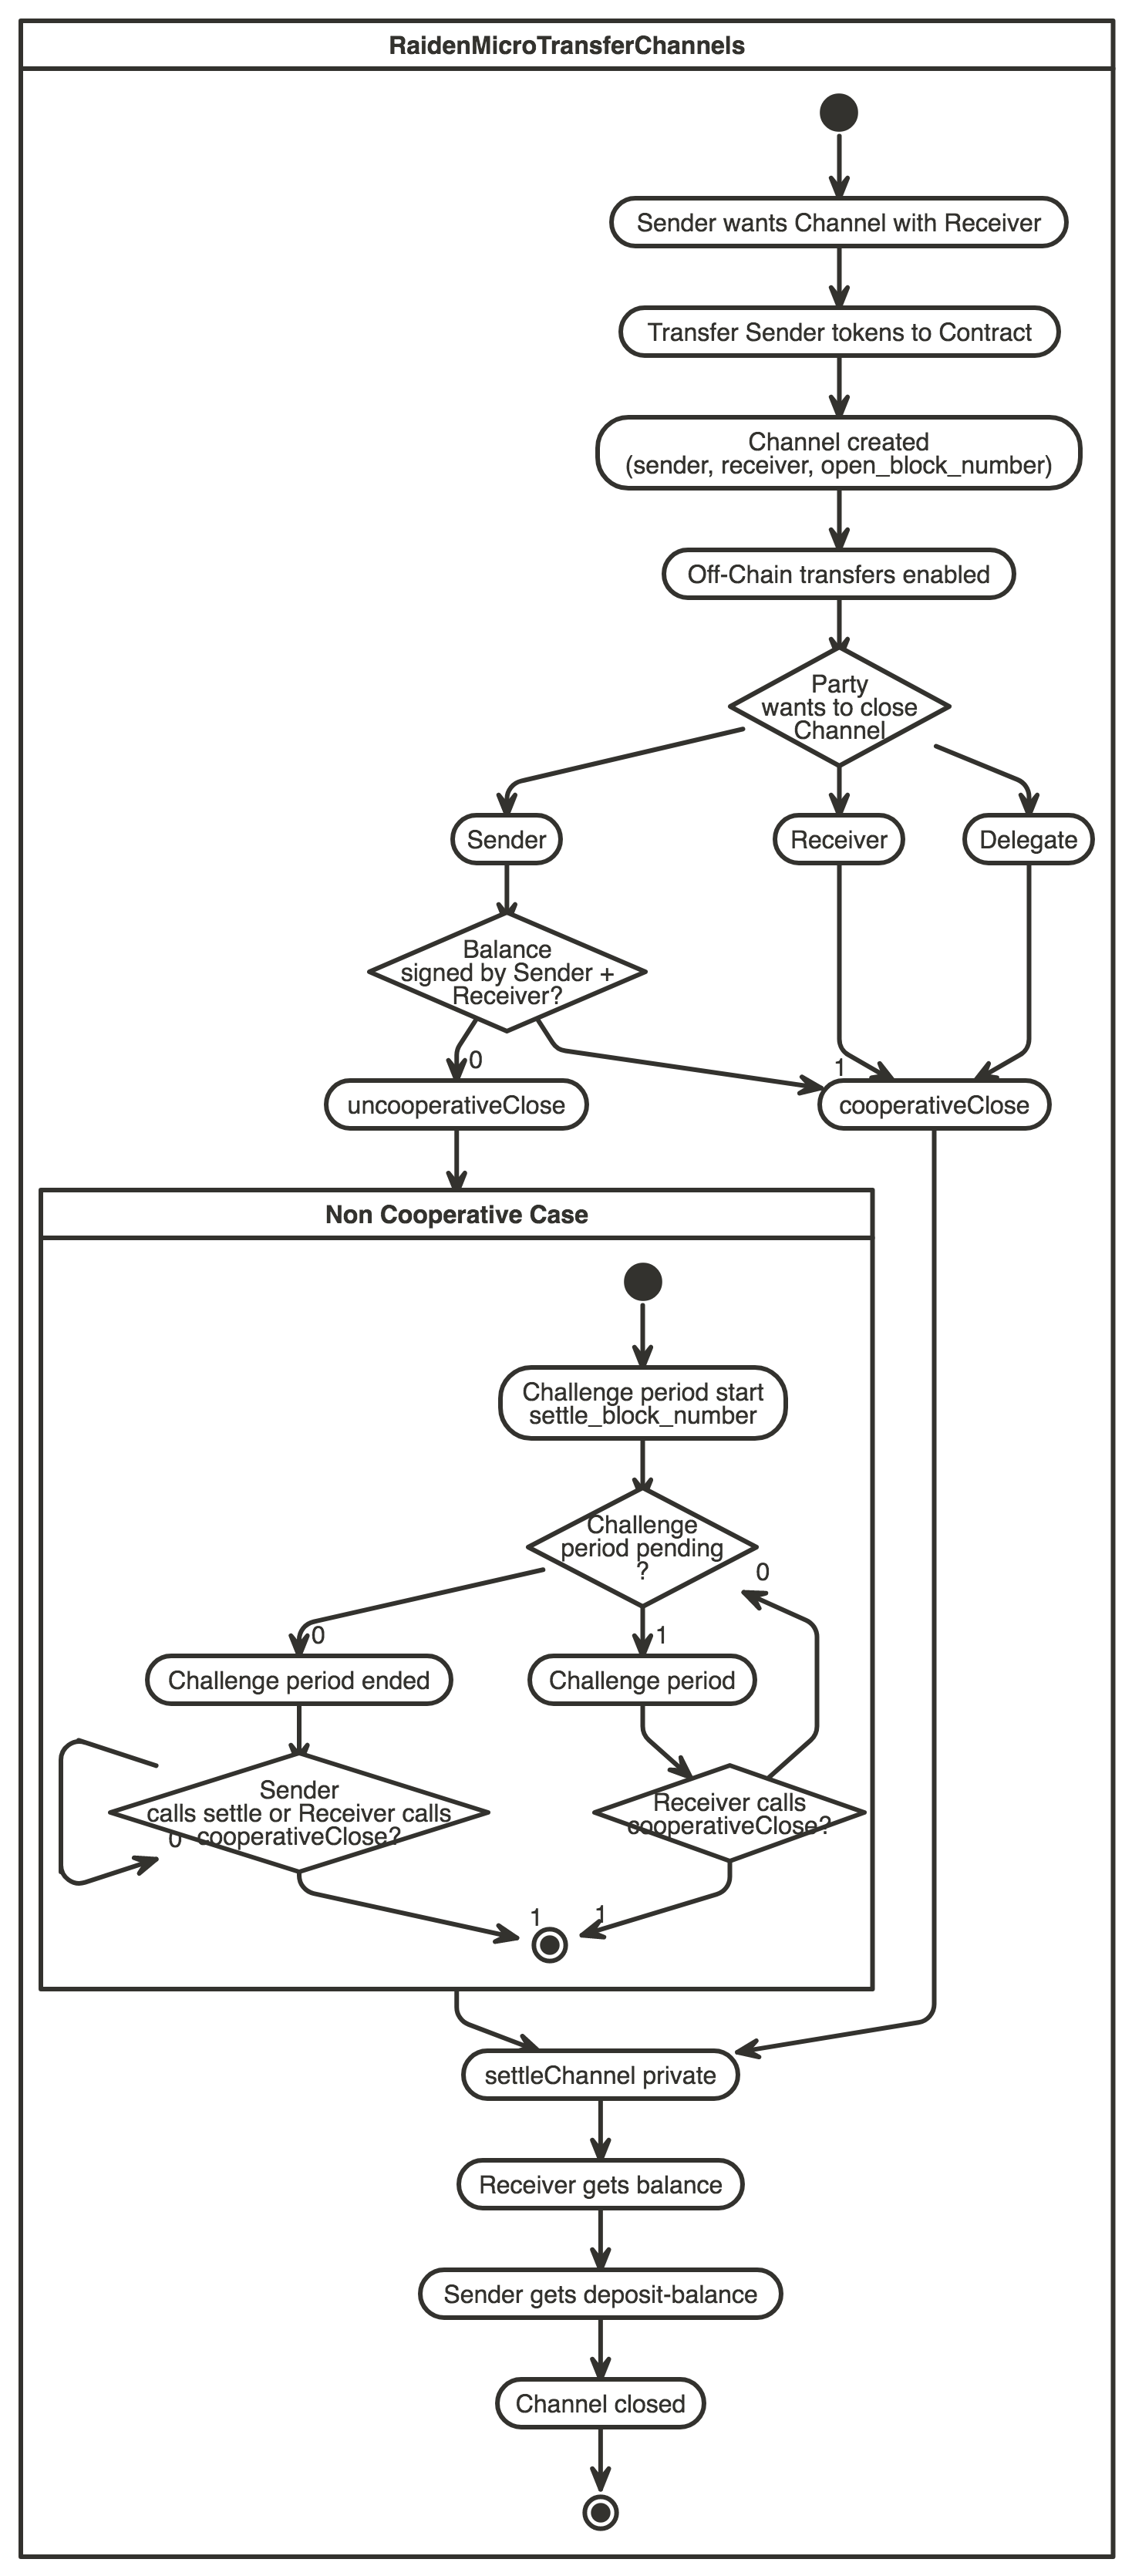
\includegraphics[width=95mm]{image/ChannelCycle.png}
 \caption{μRaidenのプロセス}
 \label{ChannelCycle}
\end{figure}
μRaidenはスマートコントラクトを使用しているので、よりフレキシブルにオフチェーン取引中の中間でトークンを引き出すことができる。
また、オンチェーンのトランザクションによってオフチェーンにデポジットしているトークン量を増やすことも可能である。
そしてERC20やERC223に準拠したEthereumネットワーク上で動くトークンに対して全てで動くように設計されている。

\section{まとめ}
この章はブロックチェーン技術全般についての仕組みやその問題点、BitcoinやEthereumの特徴などについて述べた。
途中ではトランザクションの処理の上限を緩和するための技術であるオフチェーン技術についても触れた。
また、Ethereumは最初にブロックチェーンが実装されたBitcoinよりもフレキシブルな非中央集権のコードベースで動く世界を作られる可能性を秘めていることを述べた。